\section{Experiment}

This work presents the results of several experiments, dedicated to the $^{6,7}$H studies and one reference measurement of the same reaction mechanism, performed to control all the setup parameters and to test the reliability of the obtained results.
All the experiments were conducted in at the ACCULINNA-2 fragment separator \cite{Fomichev:2018}, recently constructed in the Flerov Laboratory of Nuclear Reaction of the Joint Institute for Nuclear Research. 
In this chapter, one briefly presents the main features of the ACCULINNA-2 facility and describes in more details the experimental setups, employed for the investigations of the isotopes of interest.

\subsection{ACCULINNA-2}

The idea of the ACCULINNA-2 in-flight separator is to provide relatively low-energy RIBs of high intensity and purity. 
That is why, it is not appropriate to compare its properties with those of such large facilities as FRS \cite{geissel:1992} and SuperFRS \cite{geissel:2003,winkler:2008} at FAIR.

ACCULINNA-2 separator is not intended to compete with the new large in-flight RIB separator devices (SuperFRS
at FAIR [7,8], ARIS at FRIB [9], BigRIPS at RIKEN [11] or others [3–6], see table 1 and fig. 2) in the sense of “crude power”. 
It should complement the existing/constructed facilities in certain fields. 
Namely, ACCULINNA-2 should provide high intensity RIBs in the lowest energy range attainable for the in-flight separators. 
We emphasize the scientific importance of the corresponding field of research and consequently we choose a cost-effective technical solution for this project. 
Within a minor fraction of the total cost of the modern RIB facilities 2 it is possible to pursue world-class research due to a specific scientific focus of this instrument. 
The prime objectives of ACCULINNA-2 are to provide a good energy resolution for the beams of radioactive nuclei and high efficiency for correlation measurements. 
The latter, combined with the selection of certain reaction mechanisms and the choice of specific kinematical conditions, could provide the spin-parity identification made for the excitation spectra of the studied exotic nuclei. 
In that case, the relatively low-energy secondary beams will provide a unique position for ACCULINNA-2 between the other fragment separators. 
So far, the energies in a range of 10–40 A MeV are not so easily available at other large-scale in-flight RIB separators.

%-------------------------------------------------------------------------------
\begin{figure}[t]
	\begin{center}
		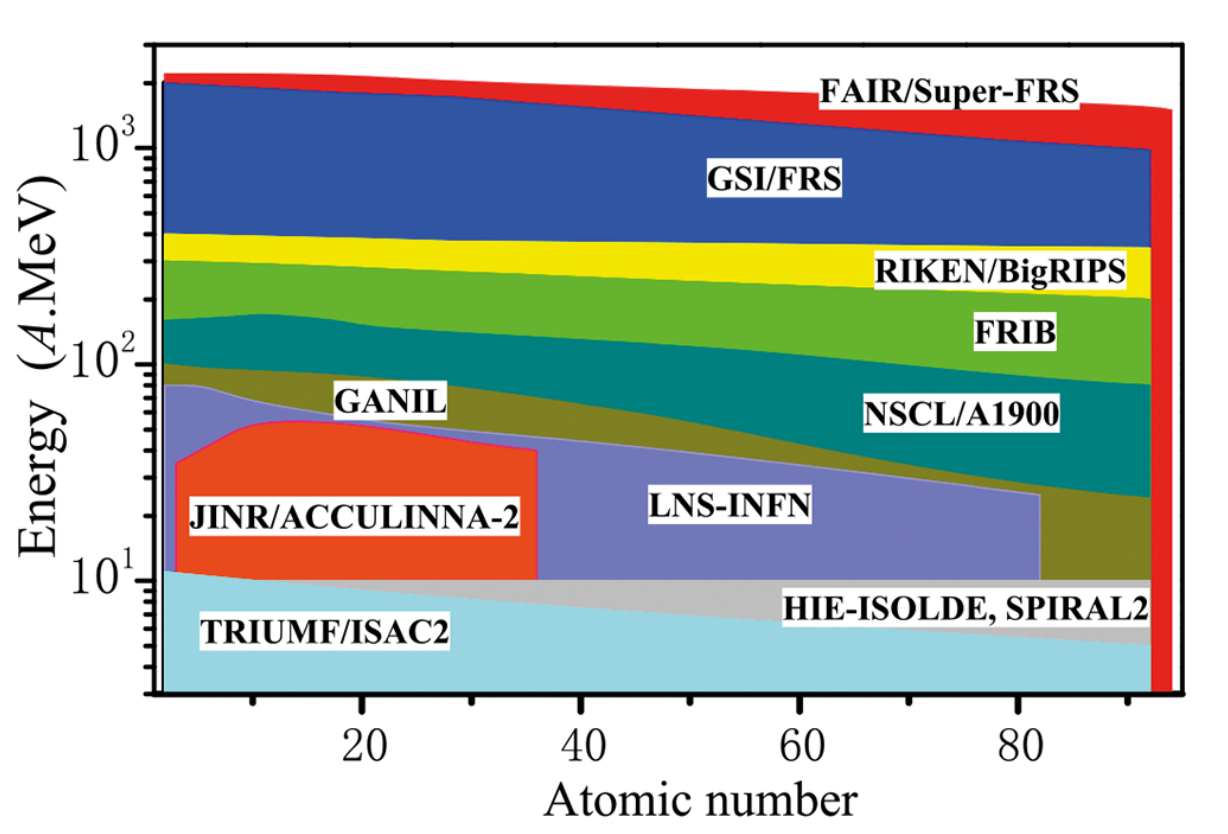
\includegraphics[width=0.7\textwidth]{figures/acculinna2_part.png}
	\end{center}
	%
	\caption{
		Landscape of the present-day facilities on the diagram where for radioactive beams, specified in terms of their atomic numbers, the available RIB energy ranges are shown.}
	%
	\label{fig:acculinna2_worldplace}
\end{figure}
%-------------------------------------------------------------------------------

%The ACCULINNA-2 facility is coupled to the U400-M cyclotron and intended for production the RIBs by in-flight method, their separation and transport. It is also can be configured to form the stable beams, derived by the cyclotron.
The ACCULINNA-2 facility is 36 meters long achromatic separator consisting of two 45-degree dipole magnets, 14 quadrupoles, eight multipoles (three octupoles and five sextupoles) and four steering magnets, see Fig.\ \ref{fig:acculinna2_scheme}.
The high intensity primary beams are delivered by the U-400M cyclotron to the rotating production target module installed in the first intermediate focal plane F1 to produce radioactive ion beams in fragmentation reactions via the in-flight method.

The target module integrates a vacuum chamber with a water cooled beryllium target mounted on rotating magnetic liquid feed through and a set of water-cooled diaphragms. 
The target module is designed to work with heating power up to 2\,kW. 
Using the combination of magnetic analysis and energy losses in achromatic wedge degrader located at the intermediate dispersive focal plane F2, the secondary ions are separated in flight. 
Then, the secondary beam is delivered into the low-background experimental area with full particle-by-particle identification.

%-------------------------------------------------------------------------------
\begin{figure}[t]
	\begin{center}
		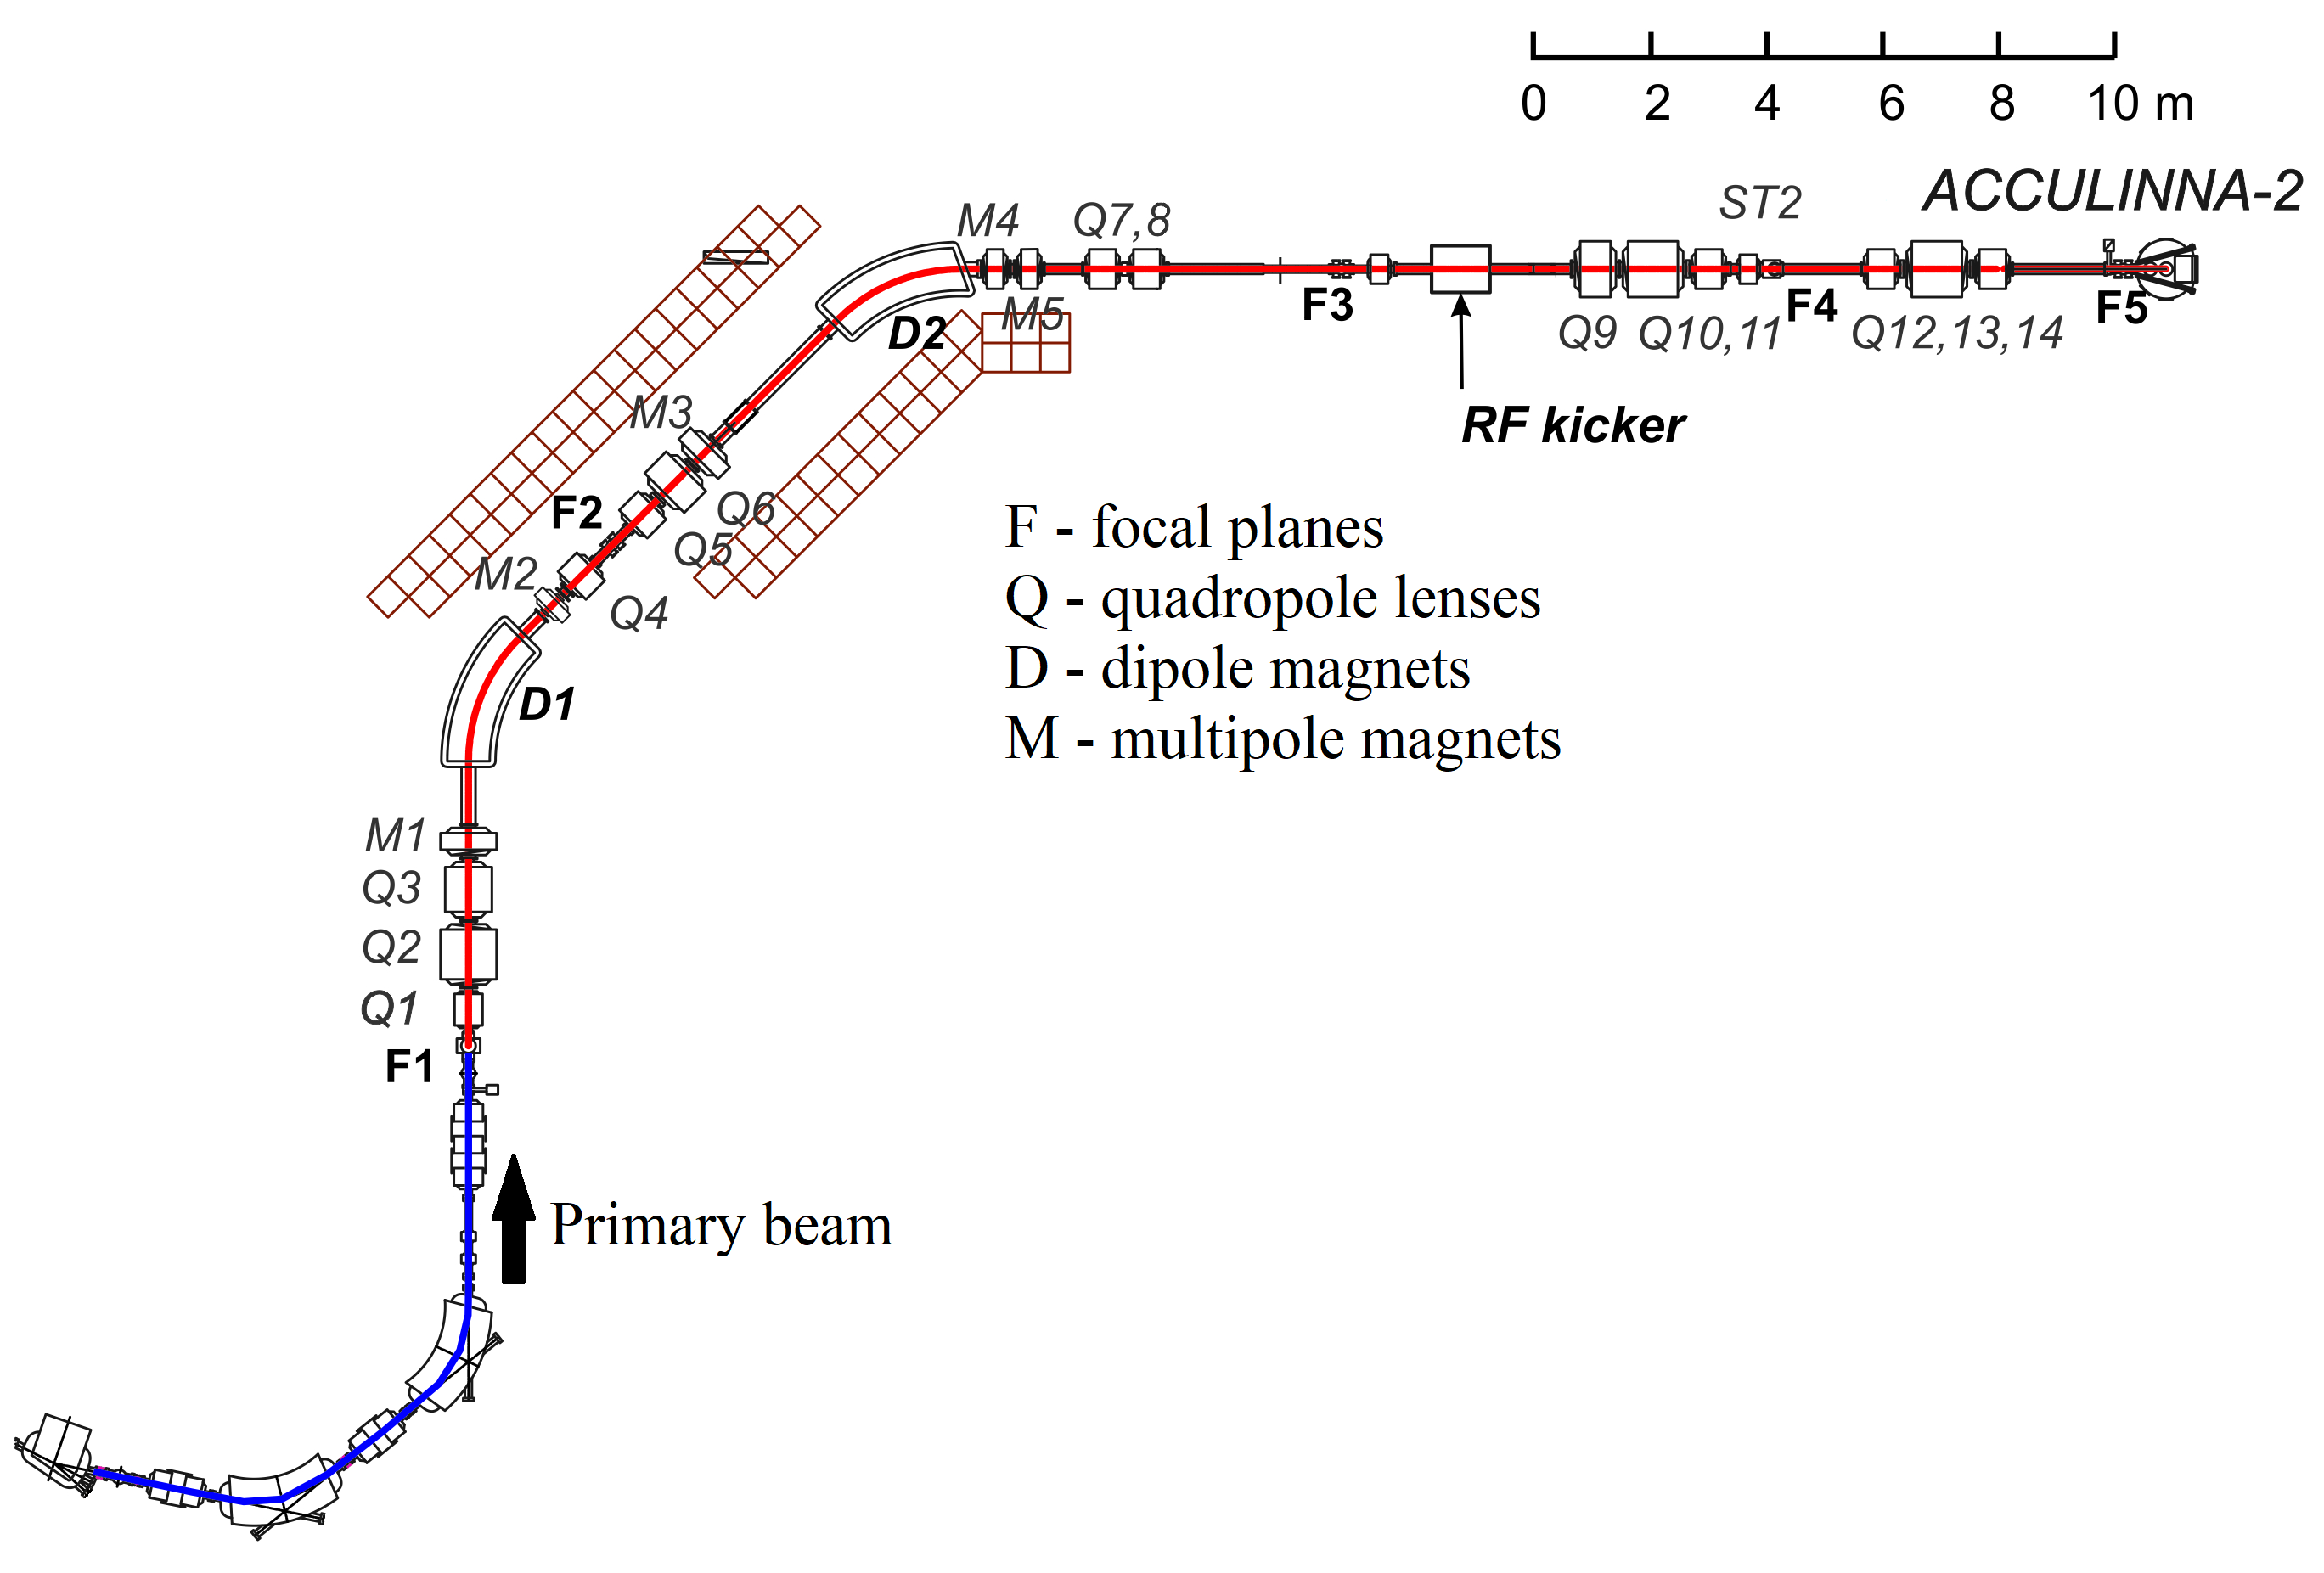
\includegraphics[width=1\textwidth]{figures/acculinna2.png}
	\end{center}
	%
	\caption{Lay-out of the fragment-separator ACCULINNA-2. F1 – the object plane; F2 – the intermediate dispersion plane; F3, F4 – the achromatic focal planes; F5 – the final focal plane.}
	%
	\label{fig:acculinna2_scheme}
\end{figure}
%-------------------------------------------------------------------------------



